\documentclass{article}

\usepackage{paper}

\usepackage[utf8]{inputenc}
\usepackage[T1]{fontenc}

\usepackage[USenglish]{babel}
\usepackage{csquotes}

\usepackage{booktabs}
\usepackage{amsfonts}
\usepackage{amsmath}
\usepackage{nicefrac}
\usepackage{microtype}
\usepackage{xcolor}
\usepackage{hyperref}
\usepackage{url}
\usepackage{graphicx}
\usepackage{float}
\usepackage{caption}
\usepackage{enumitem}

\usepackage[style=authoryear,maxbibnames=30,natbib]{biblatex}
\addbibresource{refs.bib}
\renewbibmacro{in:}{}
\DeclareDelimFormat{nameyeardelim}{\addspace}
\DeclareNameAlias{sortname}{given-family}

\usepackage[capitalize,noabbrev]{cleveref}


\title{Can Conformal Prediction Outperform Volatility Models for Financial Return Intervals? \\ A Negative Result}


\author{%
  Saurav Banna\\
  \And
  Aditya Goel\\
  \And
  Jaskeerat Singh Sarin\\
}

\begin{document}
\maketitle



\begin{abstract}
Conformal prediction (CP) offers distribution-free prediction intervals with finite-sample coverage guarantees, but relies on exchangeability --- an assumption that equity returns systematically violate through volatility clustering, fat tails, and regime shifts. Recent adaptive extensions such as Adaptive Conformal Inference (ACI), Aggregated ACI (AgACI), and Temporal Conformal Prediction (TCP) \citep{aich2026} attempt to move beyond this limitation, with TCP in particular reporting results competitive with industry-standard GARCH baselines --- motivating a deeper investigation of CP for this domain. We run a systematic comparison across three tickers and three structurally distinct crises (the 2008 Lehman collapse, the 2020 COVID crash, and the 2022 rate-hike cycle), evaluating split conformal, ACI, and AgACI paired with linear, tree-based, and neural base predictors, alongside TCP as a standalone method, and simple/naive online-adaptive baselines. Our findings are negative: rolling GARCH (Winkler 0.199) and FHS (0.242) outperform all CP methods. GARCH intervals widen immediately during crises (1.42$\times$ expansion) via the conditional variance recursion, while CP methods expand far more slowly (1.00--1.35$\times$), bounded by their calibration data distribution. TCP's reported gains are partly attributable to comparison against a static, non-rolling GARCH --- a handicapped baseline that cannot track evolving volatility. Online-updated Quantile Regression Forests match ACI-wrapped neural networks at a fraction of the complexity, and base model choice (linear AR vs.\ LSTM vs.\ Transformer) has negligible effect within any CP wrapper.
\end{abstract}

\section{Introduction}

Reliable prediction intervals for daily equity returns matter: risk desks, margin calculations, and regulatory capital all depend on quantifying how wrong a point forecast might be. The industry addresses this with GARCH \citep{engle1982,bollerslev1986}, which models conditional variance as an autoregression on past shocks, and Filtered Historical Simulation (FHS) \citep{barone2001}, which replaces the distributional assumption with empirical standardised residuals. Both are standard in practice \citep{mcneil2015}.

Conformal prediction (CP) \citep{vovk2005} produces distribution-free intervals with finite-sample coverage guarantees, but requires exchangeability --- an assumption equity returns violate through volatility clustering, fat tails, and regime shifts. Recent extensions relax this: \citet{gibbs2021} propose ACI, adjusting the miscoverage target online; \citet{zaffran2022} propose AgACI, aggregating many ACI instances; and \citet{aich2026} propose TCP, which recalibrates from a rolling window at each step. TCP was reported to match GARCH --- but we observe that the GARCH baseline in \citet{aich2026} is fitted once and held fixed, a substantial handicap that prevents it from tracking evolving volatility.

We address this directly. Our contributions are:
\begin{enumerate}[nosep,leftmargin=*]
    \item A systematic comparison of CP methods (split, ACI, AgACI with linear/tree/neural base predictors) and TCP against properly-fitted rolling GARCH and FHS across nine (ticker, crisis) pairs spanning three structurally distinct crises, using the Winkler score as the primary metric.
    \item An online extension of histogram binning and Quantile Regression Forests via per-step updates, testing whether CP's formal apparatus is necessary to match its empirical performance.
    \item A controlled re-evaluation of TCP against rolling GARCH, clarifying that TCP's reported gains are partly attributable to baseline choice and identifying the remaining structural bottleneck: CP calibration reflects a pre-crisis distributional regime that online quantile adjustment cannot fully escape.
\end{enumerate}

Our headline finding is negative: CP methods cannot outperform rolling GARCH and FHS. The gap is structural --- GARCH widens intervals through the variance recursion at every step; CP methods are bounded by their calibration residuals and expand far more slowly. The exchangeability violation in equity returns is not a technical inconvenience that adaptive CP overcomes --- it is the central obstacle, and current methods have not solved it.

\section{Related Work}

% \textbf{Industry volatility models.} \citet{engle1982} and \citet{bollerslev1986} establish GARCH, which parameterises conditional variance as \(h_t = \omega + \alpha r_{t-1}^2 + \beta h_{t-1}\), enabling one-step-ahead variance forecasts. \citet{barone2001} introduce FHS, which fits GARCH to standardise residuals then samples empirical quantiles of the standardised series, avoiding any distributional assumption on innovations. Both are standard in risk practice \citep{mcneil2015}.

\textbf{CP for non-stationary sequences.} \citet{gibbs2021} relax the exchangeability requirement by updating the target miscoverage \(\alpha_t\) online from observed coverage errors (ACI). \citet{zaffran2022} aggregate multiple ACI copies with different learning rates via an online expert algorithm to remove the need to tune the learning rate (AgACI). \citet{aich2026} propose TCP, which uses rolling-window split-conformal calibration from a trailing window of recent observations rather than a fixed pre-crisis calibration set.

\textbf{Finance-specific CP comparisons.} \citet{fantazzini2024} compares ACI against GARCH for VaR on crypto-assets, finding ACI favourable but with narrow scope (one CP variant, one tail-risk metric, non-equity assets); the paper also notes that base model complexity has little impact on CP coverage, consistent with our findings in \cref{sec:rq3}. \citet{aich2026} is most directly related: they compare TCP against a GARCH baseline with hardcoded parameters (\(\omega = 10^{-6}\), \(\alpha = 0.05\), \(\beta = 0.90\), normal innovations, no MLE), which substantially understates what a properly-specified rolling GARCH achieves. We show that rolling GARCH with Student-\(t\) innovations and monthly MLE refitting closes most of TCP's claimed gap.


\section{Methods}

\subsection{Experimental Setup}

We work on daily log-returns \(r_t = \log(P_t / P_{t-1})\) for nine (ticker, crisis) pairs: \textbf{2008 Lehman} \{AIG, GNW, MGM\}, \textbf{2020 COVID} \{MCD, MGM, AZO\}, and \textbf{2022 rate-hike} \{SNAP, NFLX, META\}. Tickers are chosen to represent sectors most exposed to each crisis. Data are sourced from \texttt{yfinance} from 2003 onward. For each pair we use a four-year training window ending twelve months before crisis onset, a six-month calibration slice, and a test window spanning six months before through six months after the exogenous crisis end. All onset and end dates are fixed a priori from documented external events to avoid circularity in adaptation-speed measurement. All methods are evaluated at nominal coverage \(1 - \alpha = 0.90\). A single refit cadence of every 21 trading days (approximately monthly) is applied to all methods that refit parameters, so the comparison is equalized on compute.

\subsection{Method Categories}

\textbf{Baselines (GARCH, FHS).} Rolling GARCH(1,1) with Student-\(t\) innovations, re-estimated on a 504-day trailing window every 21 steps via maximum likelihood using the \texttt{arch} library \citep{sheppard2022}. Intervals use the parametric \((1-\alpha/2)\) Student-\(t\) quantile of the fitted distribution applied to the one-step-ahead conditional standard deviation. FHS fits GARCH once on train-plus-calibration data and uses the empirical quantile of standardised residuals scaled by the daily forecast \(\sigma_{t+1}\).

\textbf{Simple Native Online (QRF, Hist-Bin).} Quantile Regression Forests \citep{meinshausen2006} and histogram-binning quantile lookup, initialised from training data and extended online: after each test observation the realised return is added to the stored pool (for QRF, triggering a forest refit every 21 steps). This tests whether simple adaptive strategies without a conformal layer can match CP-wrapped neural networks.

\textbf{Simple CP (LinearAR + split / ACI / AgACI).} A five-lag linear autoregression wrapped with three conformal methods. Split-CP uses a fixed calibration quantile. ACI updates \(\alpha_t \leftarrow \alpha_t + \gamma(\alpha - \mathbf{1}[\text{miss}_t])\) with \(\gamma = 0.01\). AgACI runs \(K=12\) ACI instances over a geometric grid of learning rates, aggregated via exponential weights.

\textbf{Complex CP (LSTM, Transformer + split / ACI / AgACI).} The same three wrappers applied to a single-layer LSTM (50 hidden units) and a one-layer Transformer encoder (\(d_{\text{model}}=32\), 4 heads), both trained with Adam, max 50 epochs, early stopping. This tests whether neural base predictor complexity helps within the CP framework.

\textbf{TCP (daily refit).} \citet{aich2026} propose TCP: rolling split-conformal on a trailing 252-day window split into 192 train and 60 calibration rows, with two quantile gradient-boosted machines as the base predictor. The conformal threshold \(C_t\) is recomputed from the most recent 60-day calibration slice at every step. Because this refitting cadence is the core adaptation mechanism, we evaluate TCP at its native daily refit rather than the shared 21-step cadence.

\subsection{Metrics}

\textbf{Winkler score} \citep{winkler1972,gneiting2007} is our primary metric:
\[
  W_t = (u_t - l_t) + \tfrac{2}{\alpha}\max(l_t - r_t, 0) + \tfrac{2}{\alpha}\max(r_t - u_t, 0).
\]
It jointly penalises interval width and miscoverage at a 20:1 ratio (\(\alpha = 0.10\)), preventing a method from achieving a good score purely through over-widening. Lower is better.

\textbf{Marginal coverage} is the empirical proportion of test days where \(r_t \in [l_t, u_t]\). The nominal target is 0.90.

\textbf{Crisis coverage} is marginal coverage restricted to the exogenous crisis window, measuring interval quality when it matters most.

\textbf{Coverage gap} is \(\text{Cov}_{\text{low-vol}} - \text{Cov}_{\text{high-vol}}\), where the high-volatility mask is the top quartile of 20-day rolling realised variance computed once per asset over the full sample. A large gap means the method masks crisis failures behind calm-period success.

\textbf{Width expansion ratio} is mean crisis-period width divided by mean overall width. A ratio of 1.00 means the interval did not widen during the crisis at all.


\section{Results}

\cref{tab:main} summarises all methods averaged across the nine ticker-regime cells, sorted by Winkler score.

\begin{table}[t]
\caption{Main results averaged across nine ticker-regime cells, sorted by Winkler score (lower is better). \textbf{Gap} is $\text{Cov}_{\text{low-vol}} - \text{Cov}_{\text{high-vol}}$ (lower = more consistent). \textbf{Exp.} is crisis-period width divided by overall width. Nominal target: coverage 0.90, gap 0.00. $\dagger$ TCP uses daily refit; all other methods use 21-step refit cadence.}
\label{tab:main}
\centering
\small
\setlength{\tabcolsep}{5pt}
\begin{tabular}{llccccccc}
\toprule
Model & Wrapper & Marg.\ Cov & Cov.\ Crisis & Gap & Winkler & Width & Exp. \\
\midrule
GARCH-Roll & Native & 0.949 & 0.895 & 0.047 & \textbf{0.199} & 0.156 & 1.42$\times$ \\
FHS        & Native & 0.915 & 0.857 & 0.077 & 0.242 & 0.164 & 1.56$\times$ \\
TCP$^\dagger$ & Daily  & 0.897 & 0.813 & 0.082 & 0.281 & 0.177 & 1.36$\times$ \\
\midrule
LSTM       & ACI    & 0.820 & 0.668 & 0.174 & 0.305 & 0.109 & 1.18$\times$ \\
LinAR      & ACI    & 0.821 & 0.668 & 0.164 & 0.307 & 0.110 & 1.19$\times$ \\
QRF        & Online & 0.801 & 0.671 & 0.155 & 0.309 & 0.124 & 1.35$\times$ \\
LSTM       & AgACI  & 0.811 & 0.651 & 0.201 & 0.310 & 0.105 & 1.15$\times$ \\
Transformer & ACI   & 0.819 & 0.664 & 0.178 & 0.311 & 0.110 & 1.20$\times$ \\
Hist-Bin   & Online & 0.750 & 0.565 & 0.235 & 0.344 & 0.094 & 1.12$\times$ \\
LSTM       & Split  & 0.694 & 0.462 & 0.312 & 0.399 & 0.072 & 1.00$\times$ \\
\bottomrule
\end{tabular}
\end{table}

\subsection{RQ1: Can CP outperform GARCH and FHS?}
\label{sec:rq1}

No. Rolling GARCH achieves a Winkler score of 0.199 and FHS 0.242. The best conformal method, LSTM~$\times$~ACI, scores 0.305 -- 53\% worse than GARCH. This gap is consistent across all three crisis regimes (see \cref{app:regime}). GARCH and FHS also maintain near-nominal marginal coverage (0.949 and 0.915 respectively) with the smallest coverage gaps (0.047 and 0.077), meaning their coverage is consistent across high- and low-volatility periods. ACI/AgACI variants drop to 0.81--0.82 marginal coverage (gaps 0.16--0.20), and split-CP to 0.68--0.69 (gaps over 0.30).

\subsection{RQ2: Why -- the width adaptation mechanism}
\label{sec:rq2}

\cref{fig:timeline} illustrates this on MCD (2020 COVID): GARCH intervals expand and contract with volatility, while LSTM~$\times$~ACI stays narrow and accumulates misses through the crash.
\begin{figure}[t]
\centering
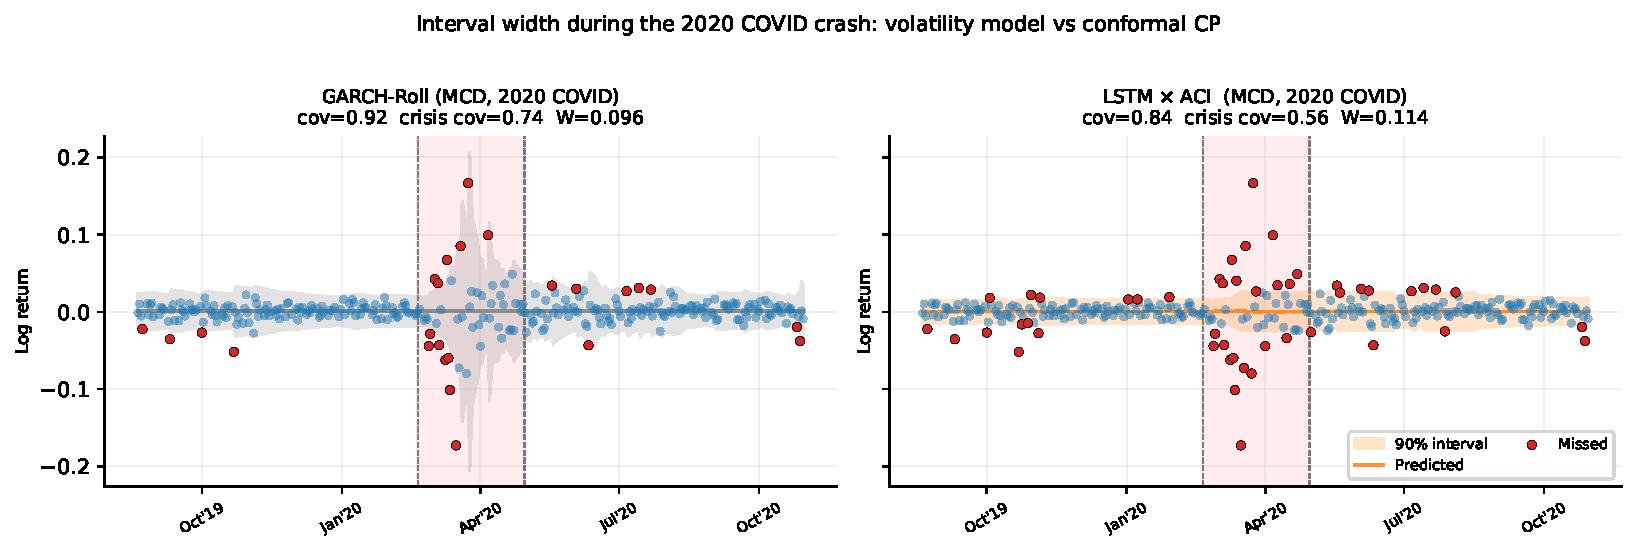
\includegraphics[width=\linewidth]{figures/timeline_comparison.pdf}
\caption{Prediction intervals for McDonald's (MCD) through the 2020 COVID crash.
  Left: GARCH-Roll intervals widen immediately as volatility spikes and recover afterward
  (crisis coverage 0.74, Winkler 0.096).
  Right: LSTM $\times$ ACI intervals stay narrow throughout the crash, accumulating misses
  (crisis coverage 0.56, Winkler 0.114).
  Red shading marks the exogenous crisis window. Red dots are missed observations.}
\label{fig:timeline}
\end{figure}

\cref{fig:dumbbell} quantifies this across all methods. GARCH expands its intervals 1.42$\times$ during crisis periods, FHS 1.56$\times$. Split-CP methods do not expand at all (1.00$\times$, open and filled circles overlap). ACI and AgACI variants expand only modestly (1.15--1.20$\times$).

The mechanism is structural. GARCH intervals are \(\hat{\mu} \pm z \cdot \sigma_{t+1}\) where \(\sigma_{t+1}\) is computed from the variance recursion \(h_{t+1} = \omega + \alpha r_t^2 + \beta h_t\) every single step. One large crisis return on day \(t\) directly feeds into \(\sigma_{t+1}\) the next day. Split-CP intervals are \(\hat{\mu} \pm \hat{q}\) where \(\hat{q}\) is a fixed quantile of pre-crisis calibration residuals: no mechanism exists for it to grow. ACI adjusts \(\alpha_t\) downward after each miss, which shifts to a higher quantile of the same calibration residual distribution -- but that distribution was fit on calm pre-crisis data, so the ceiling on interval expansion is set by the maximum calibration residual ever observed, which is far smaller than crisis-period returns.

\begin{figure}[t]
\centering
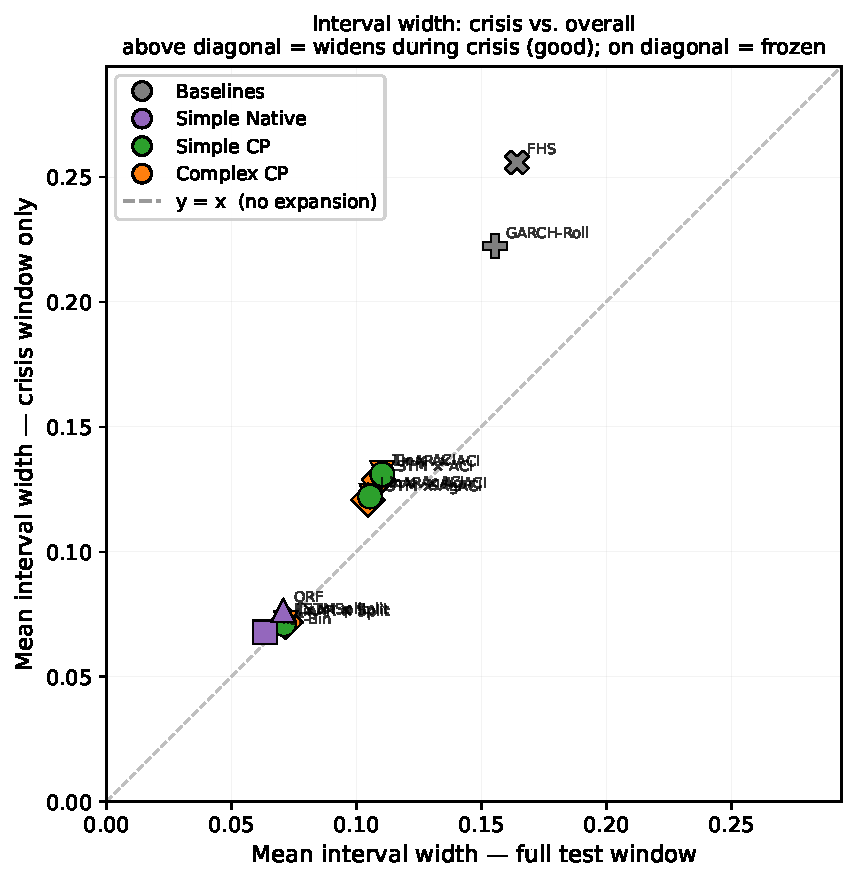
\includegraphics[width=0.75\linewidth, height=0.35\textheight]{figures/width_adaptation.pdf}
\caption{Crisis width expansion across all methods. Open circles mark mean interval width over the full test window; filled circles mark mean width during the crisis window only. Line length is the absolute expansion; the ratio is labelled right. GARCH and FHS (gray) have the longest lines. Split-CP methods (bottom three rows) have dots that overlap exactly at 1.00$\times$.}
\label{fig:dumbbell}
\end{figure}

Adaptation speed tells the same story. We measure \(T_{\text{recovery}}\): trading days from crisis onset until rolling 20-day coverage reaches 0.85 for five consecutive days. GARCH recovers immediately (\(T_{\text{recovery}} = 0\), coverage never drops below threshold). FHS recovers within 4 days on average. QRF-Online takes approximately 27 days, ACI variants 42--47 days, and split-CP methods rarely recover at all within the crisis window (mean \(T_{\text{recovery}} > 50\) days, recovery rate 44--56\%). The ordering mirrors width expansion: methods that widen faster also recover coverage faster.

\subsection{RQ3: Base model complexity does not help}
\label{sec:rq3}

Within any conformal wrapper, base model complexity makes almost no difference. LSTM~$\times$~ACI (0.305), LinAR~$\times$~ACI (0.307), and Transformer~$\times$~ACI (0.311) are statistically indistinguishable. The same pattern holds for AgACI and split. This finding is consistent with \citet{fantazzini2024}, who observe a similar insensitivity to model choice for CP on crypto-assets. The conformal calibration mechanism, not the base predictor's accuracy, determines interval quality.

\subsection{RQ4: Simple online methods match CP-wrapped neural networks}
\label{sec:rq4}

The previous finding has a direct consequence: online QRF without any conformal layer scores 0.309 Winkler, matching LSTM~$\times$~ACI (0.305). Online Hist-Bin (0.344) also outperforms split-CP (0.399--0.408). The online adaptation matters; the conformal wrapper on top of a neural network does not add meaningful value once the calibration data has drifted. QRF's relative advantage over Hist-Bin reflects the fact that the leaf-weighting structure gives smoother quantile estimates as the lag-feature distribution shifts into a crisis regime.

\cref{fig:qrf_timeline} shows this on MCD during the 2020 COVID crash: QRF-Online's expanding leaf pool widens intervals to 1.35$\times$ while LSTM~$\times$~Split stays frozen at 1.00$\times$.

\begin{figure}[t]
\centering
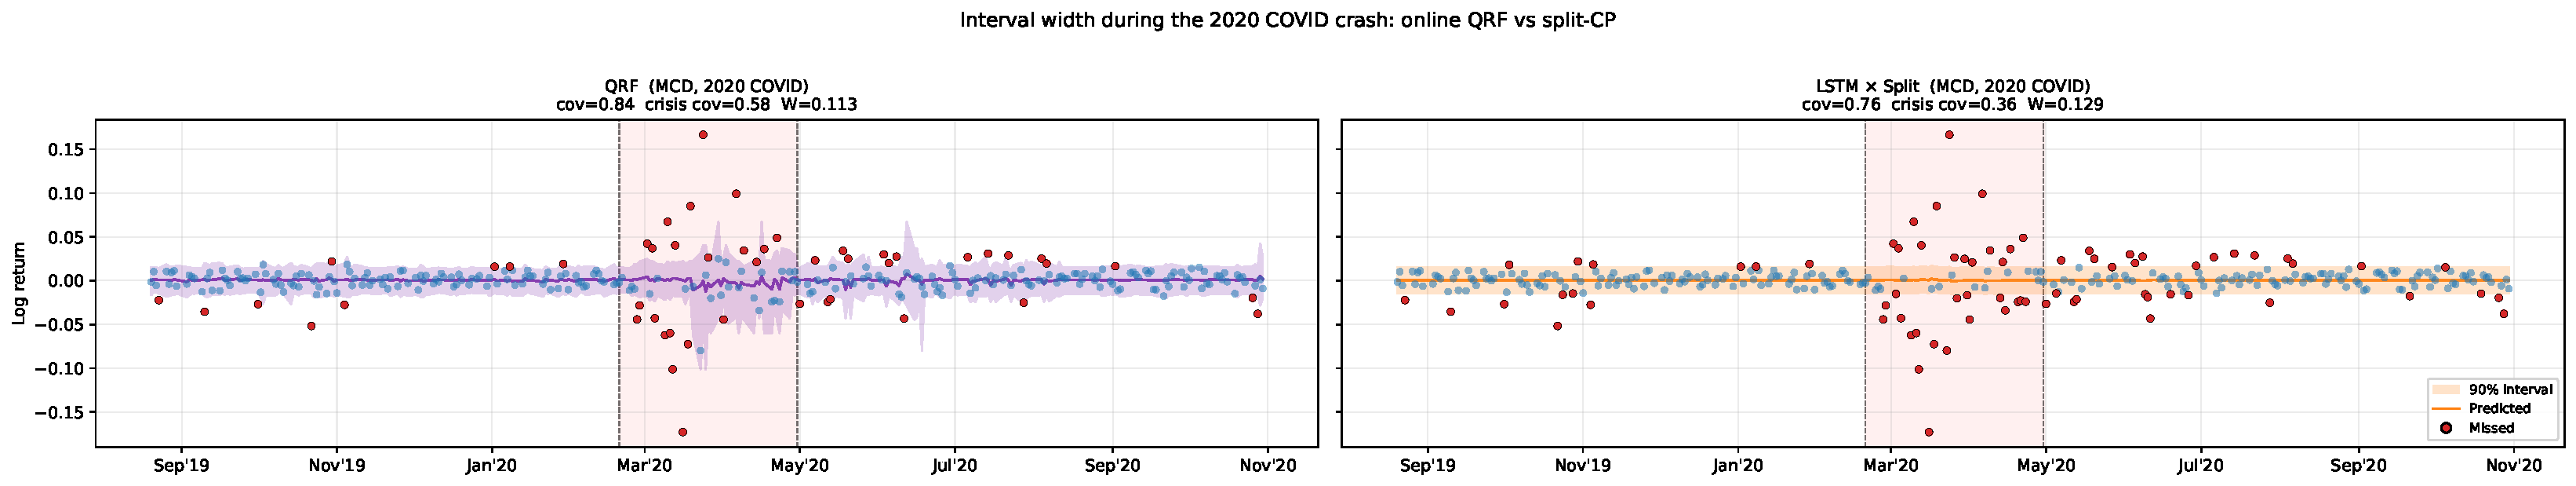
\includegraphics[width=\linewidth]{figures/timeline_qrf_online.pdf}
\caption{QRF-Online (left) expands intervals during the 2020 COVID crash via its online-adapted leaf pool (1.35$\times$ expansion), matching LSTM~$\times$~ACI at a fraction of the complexity. LSTM~$\times$~Split (right) is frozen at 1.00$\times$, accumulating missed observations (red dots) throughout the crisis window (red shading).}
\label{fig:qrf_timeline}
\end{figure}

\subsection{RQ5: TCP as a partial fix}
\label{sec:rq5}

TCP with daily recalibration (Winkler 0.281) outperforms every standard CP method while maintaining near-nominal marginal coverage (0.897). It achieves this by replacing the frozen calibration set with a rolling 60-day window: after 30 days of a crisis, \(C_t\) is estimated from 30 actual crisis observations, so the ceiling on interval width is reset to match the current regime. This removes the hard cap that limits ACI and AgACI.

However, TCP still falls behind GARCH (0.199) and FHS (0.242). First, TCP's rolling window fills with crisis data gradually: on day 1, \(C_t\) is still estimated from 60 pre-crisis rows, so the window must fill entirely before \(C_t\) reflects the new regime. GARCH's variance recursion is current as of yesterday's return with no lag (\cref{fig:tcp_timeline} illustrates this entry lag). Second, TCP's calm-period intervals are wider than needed (0.177 vs GARCH's 0.156), because the empirical quantile of a 60-day rolling window is noisier than the parametric GARCH form.

\begin{figure}[t]
\centering
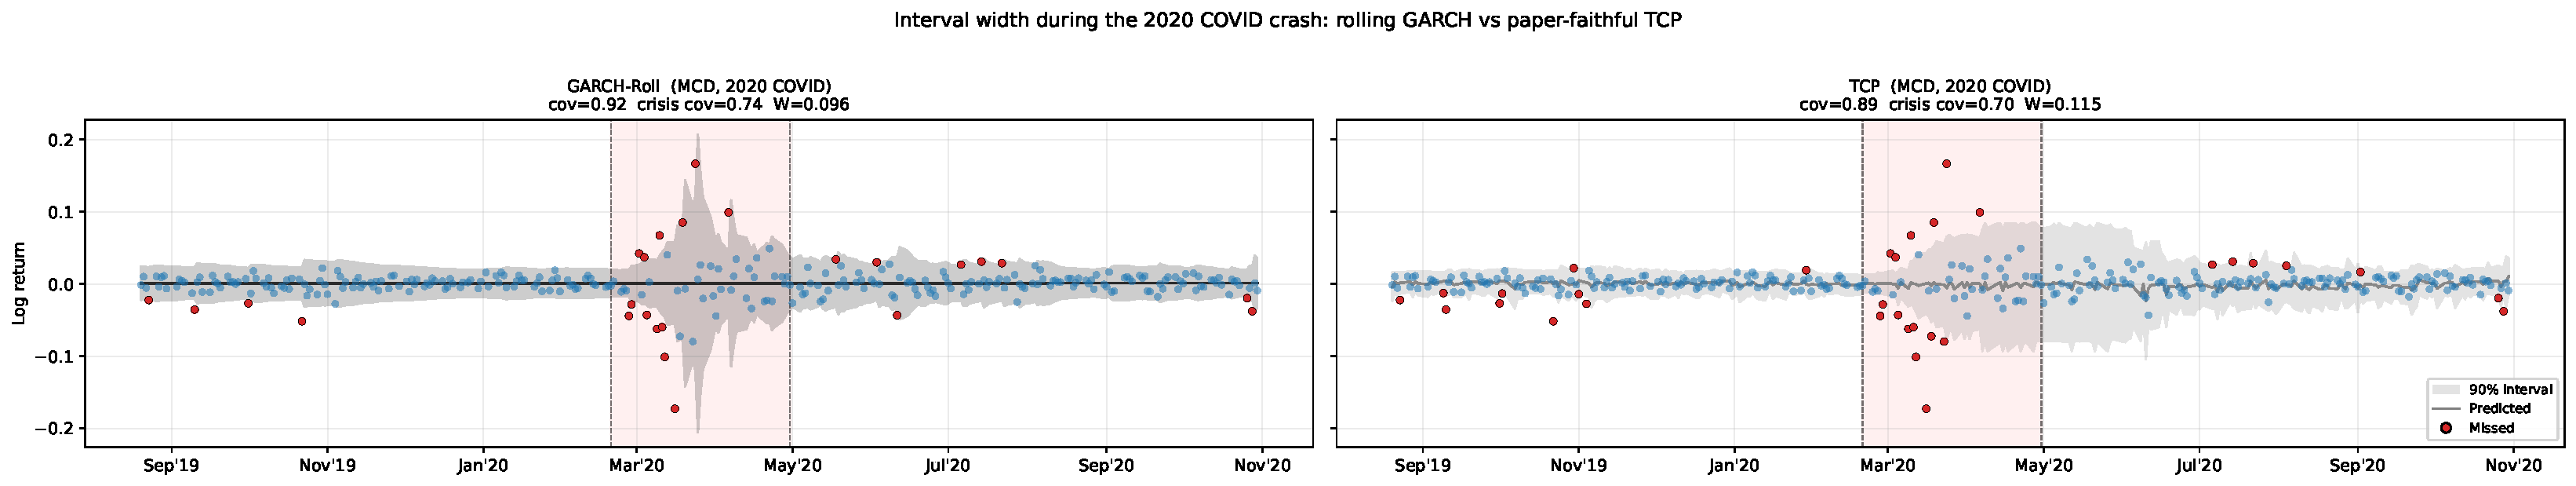
\includegraphics[width=\linewidth]{figures/timeline_tcp_vs_garch.pdf}
\caption{GARCH-Roll (left) widens immediately at crisis onset and contracts quickly afterward. TCP (right) widens gradually as the 60-day calibration window absorbs crisis returns, lagging GARCH's response by several weeks.}
\label{fig:tcp_timeline}
\end{figure}

Critically, the TCP paper \citep{aich2026} compares against a hardcoded GARCH with non-estimated parameters (\(\omega=10^{-6}\), \(\alpha=0.05\), \(\beta=0.90\), normal innovations, no MLE fitting), which substantially understates what a properly-specified rolling GARCH can achieve. Our rolling GARCH with Student-\(t\) innovations and monthly MLE refitting closes most of the gap that \citealt{aich2026} attribute to TCP's design advantage, reframing TCP's contribution as a partial improvement over standard CP rather than a competitor to industry baselines.

\section{Discussion}

\textbf{Summary.} CP methods, even adaptive variants, cannot outperform properly-calibrated rolling GARCH and FHS for daily equity return intervals across crisis regimes. The failure is structural and can be stated concisely: conformal scores are \emph{backward-looking} --- they are quantiles of a stored residual distribution that can only change as new observations accumulate --- while GARCH is \emph{forward-looking} --- the variance recursion \(h_{t+1} = \omega + \alpha r_t^2 + \beta h_t\) is a one-step-ahead forecast that incorporates yesterday's shock immediately. This asymmetry means GARCH adapts at the speed of the data, while CP adapts at the speed of the calibration window.

\textbf{Limitations.} Three tickers per regime is a small basket; a broader cross-section would tighten variance. The 2008 window dropped AIG and GNW for GARCH because the pre-crisis period caused MLE to converge to a near-unit-root solution, reflecting genuine financial instability rather than an implementation issue. TCP's daily refit is compared against GARCH's monthly parameter refit, though GARCH's variance recursion adapts every step regardless.

\textbf{Future work.} The most direct fix for CP in this setting would be to use GARCH-standardised residuals as conformal scores rather than raw residuals, combining the volatility model's width adaptation with the distribution-free coverage guarantee. Our codebase supports this as a wrapper-level change without modifying the underlying models.

\printbibliography
\appendix

\section{Supplementary Material}
\label{app:info}

\subsection*{Source Code}

Code, interval CSVs, and the full metrics table are available at \url{https://github.com/agoel25/conformalQuant}.

\subsection*{Reproduction}

All results are fully reproducible from the project root:
\begin{verbatim}
python scripts/run_grid.py        # generates all interval CSVs (~15 min CPU)
python scripts/build_artifacts.py # metrics_long.csv + paper figures
\end{verbatim}

\subsection*{Experimental timeline}

\begin{figure}[h]
\centering
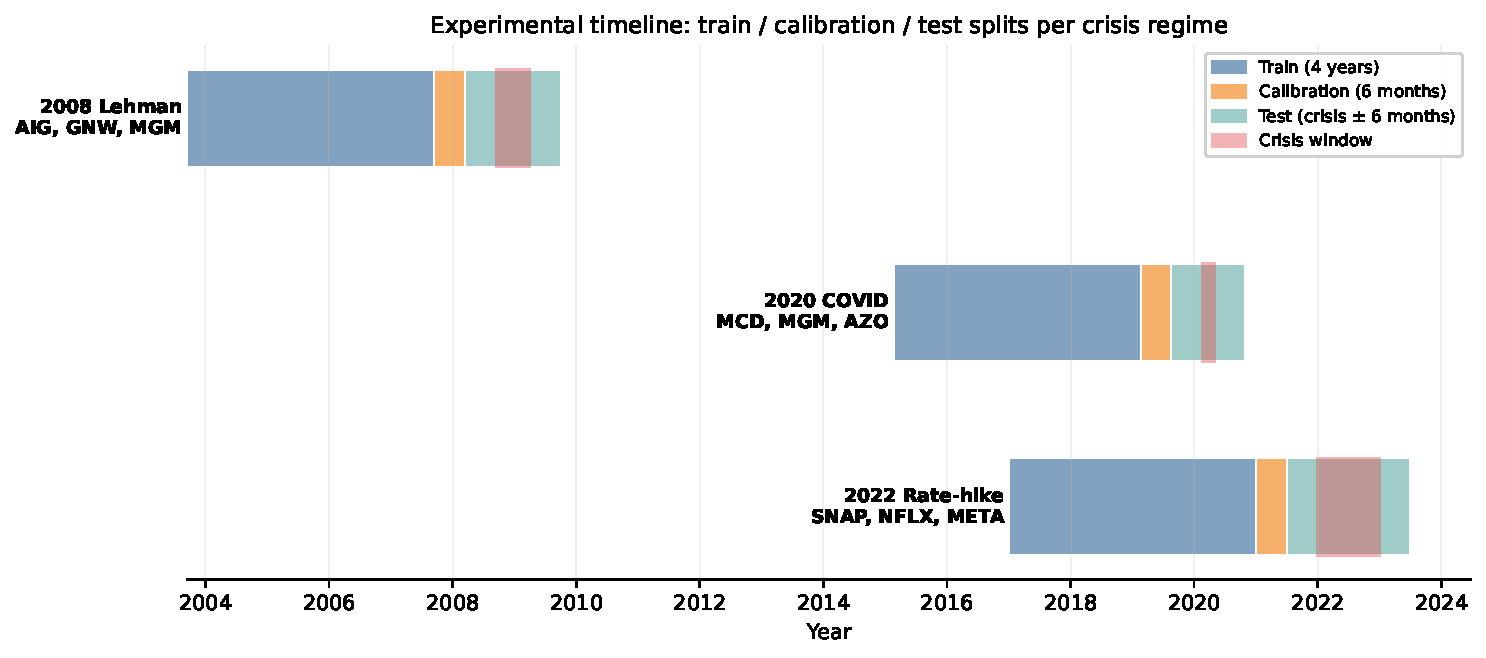
\includegraphics[width=\linewidth]{figures/crisis_timeline.pdf}
\caption{Train, calibration, and test windows for each crisis regime. Tickers are chosen to represent sectors most exposed to each crisis. Crisis onset and end dates are fixed from documented external events to avoid circularity in adaptation-speed measurement.}
\label{fig:crisis_timeline}
\end{figure}

\subsection*{Crisis window validation}

Our crisis onset and end dates are fixed exogenously from documented market events (Lehman bankruptcy filing, S\&P~500 pre-crash peak, Fed rate-hike cycle start) rather than derived from the return series. This avoids circularity: if we detected regime changes from the data, our adaptation-speed metric would be measuring how quickly each method responds to a threshold we chose to match the data. \cref{fig:regime_cumreturn,fig:regime_vol} confirm that the exogenous dates align with actual drawdowns and volatility spikes for every ticker in our crash baskets.

\begin{figure}[h]
\centering
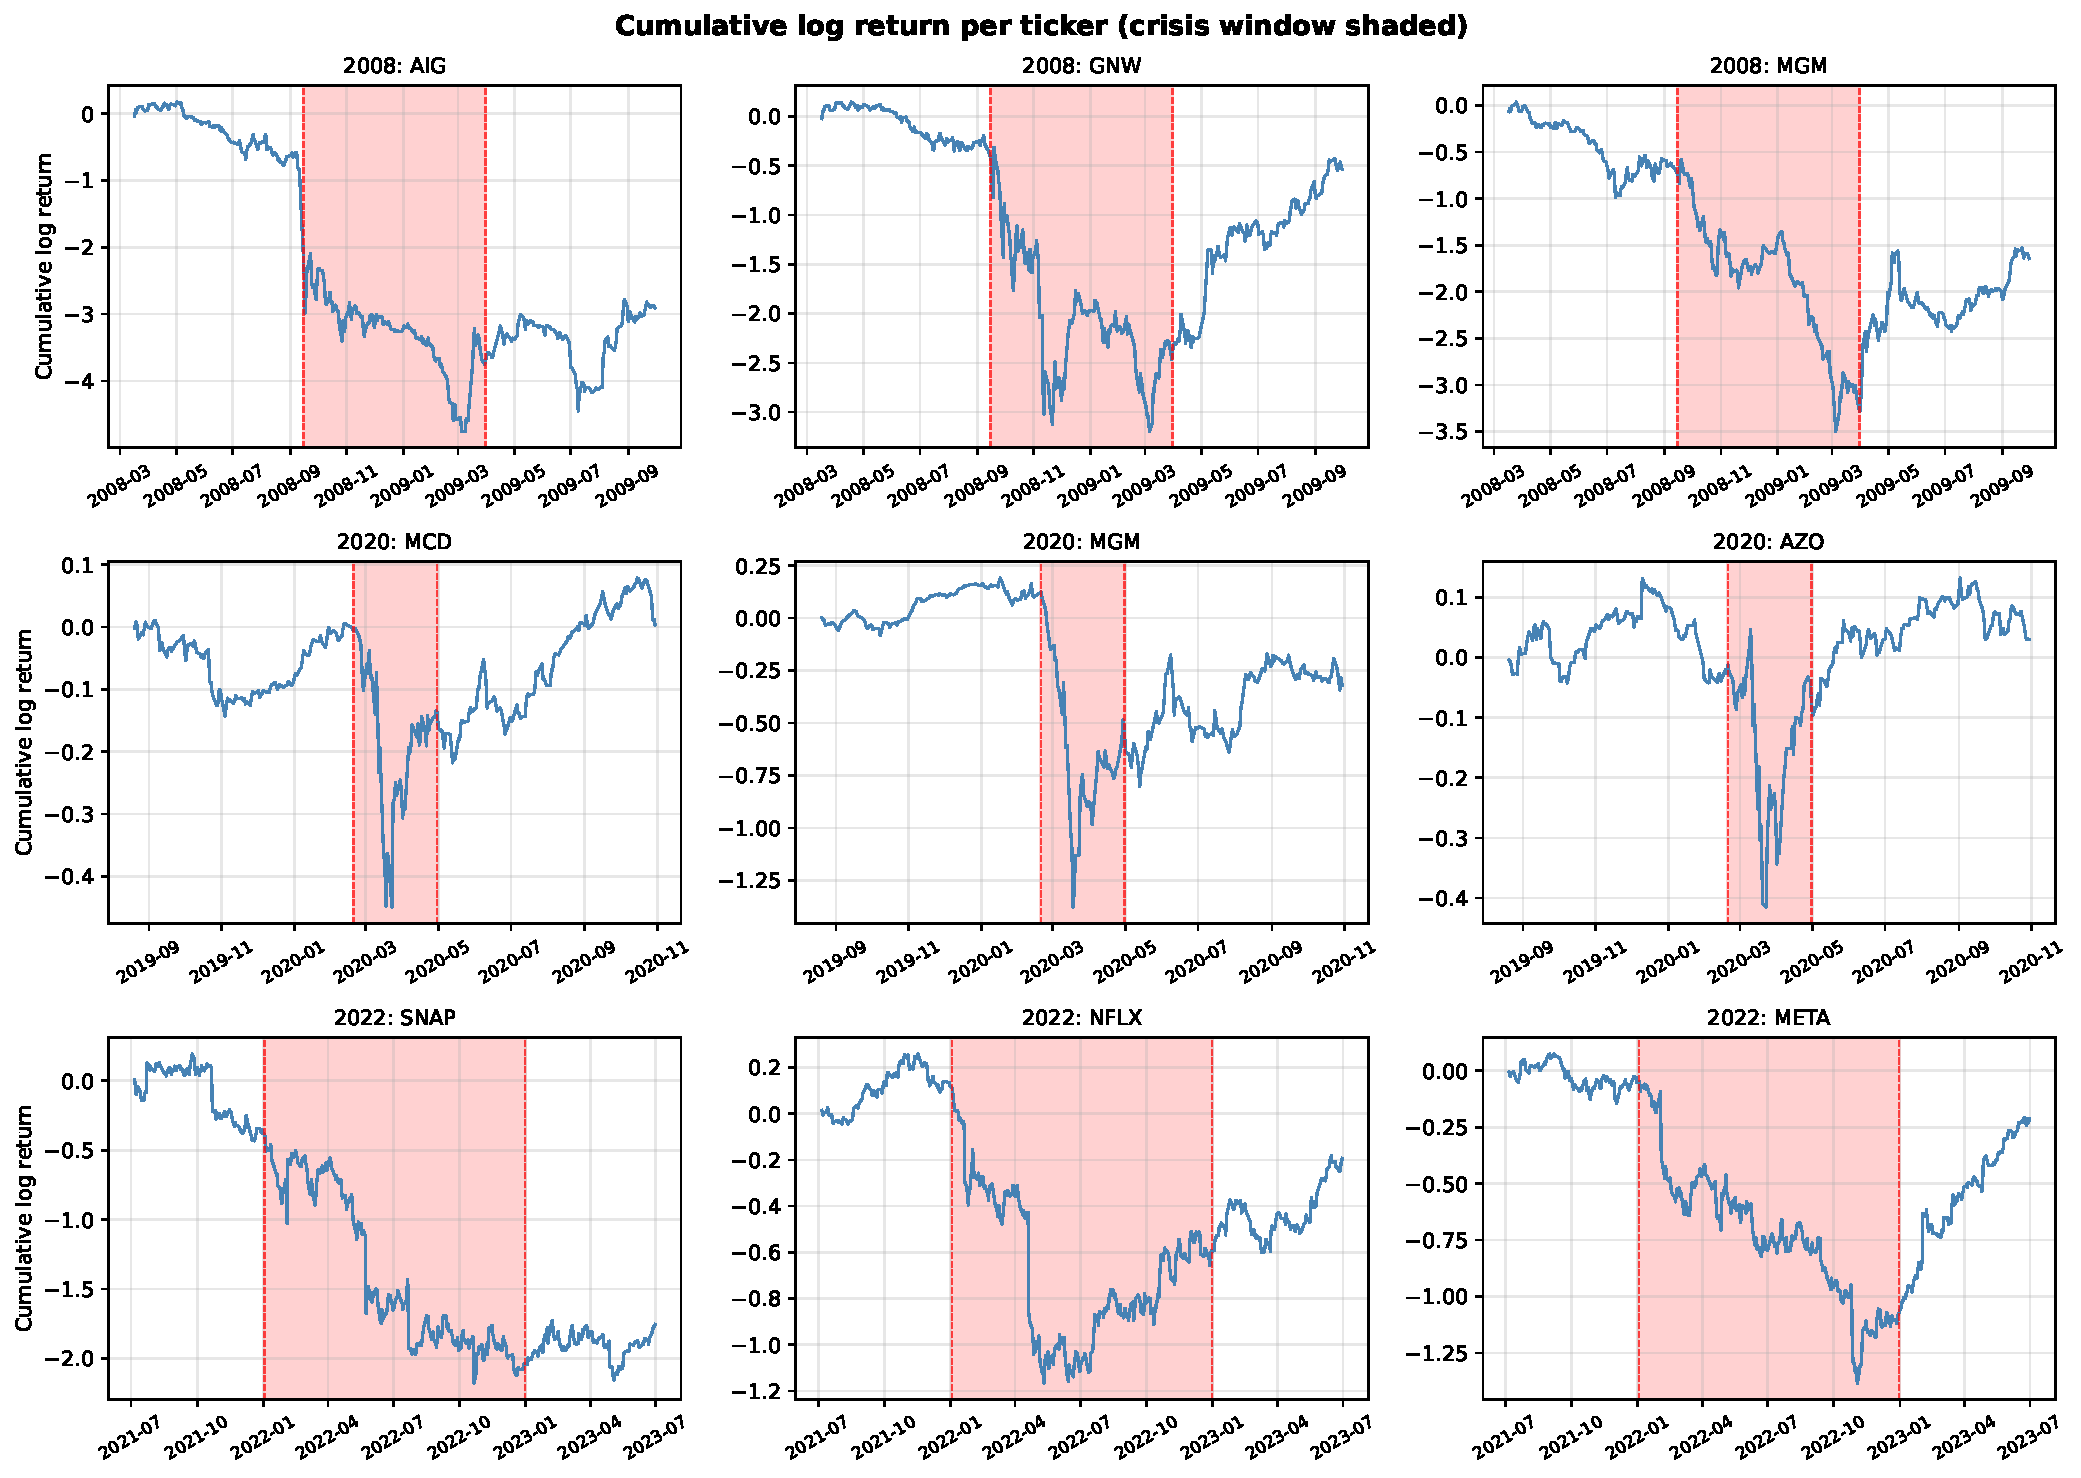
\includegraphics[width=0.95\linewidth]{figures/regime_cumreturn.pdf}
\caption{Cumulative log return per ticker. Red shading = exogenous crisis window. Every ticker shows a clear drawdown inside the shaded region.}
\label{fig:regime_cumreturn}
\end{figure}

\begin{figure}[h]
\centering
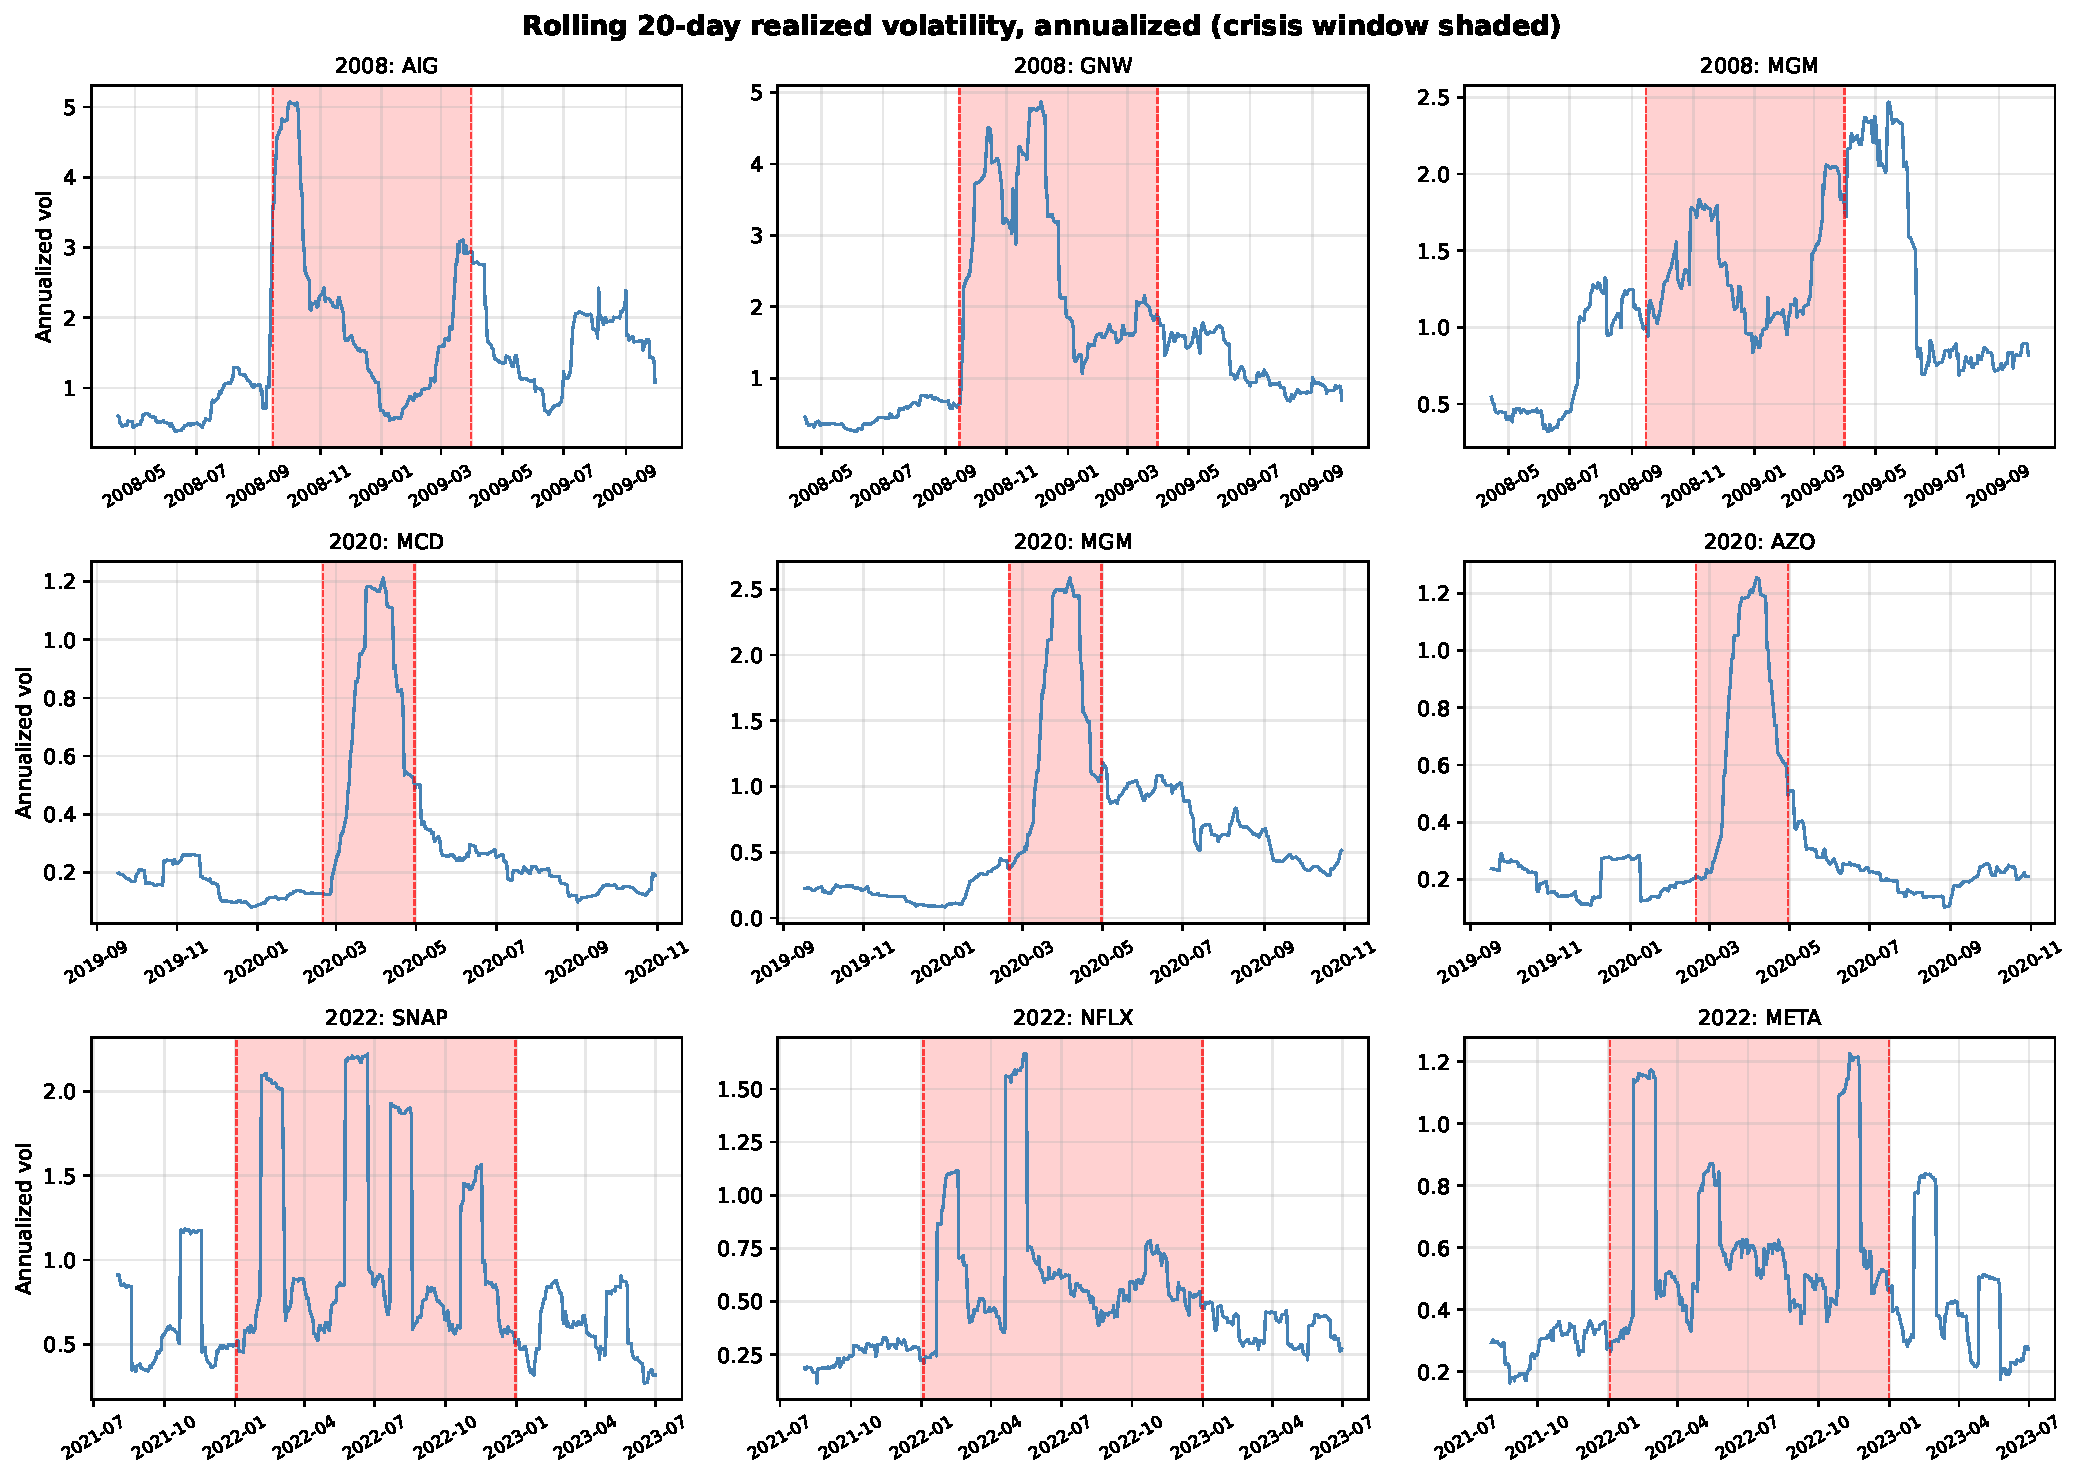
\includegraphics[width=0.95\linewidth]{figures/regime_volatility.pdf}
\caption{Rolling 20-day annualized realized volatility. Volatility spikes sharply inside the crisis window for all tickers, confirming the fixed dates capture genuine regime shifts.}
\label{fig:regime_vol}
\end{figure}

\subsection*{Per-regime breakdown}

\begin{table}[h]
\caption{Marginal coverage by crisis regime for selected methods, averaged over the three tickers in each regime. Full 114-row results are in \texttt{results/metrics\_long.csv}.}
\label{app:regime}
\centering
\small
\begin{tabular}{llccc}
\toprule
Model & Wrapper & 2008 & 2020 & 2022 \\
\midrule
GARCH-Roll & Native & 0.933 & 0.934 & 0.970 \\
FHS        & Native & 0.912 & 0.908 & 0.924 \\
TCP$^\dagger$ & Daily & 0.886 & 0.897 & 0.908 \\
LinAR      & ACI    & 0.726 & 0.841 & 0.898 \\
LSTM       & ACI    & 0.714 & 0.848 & 0.898 \\
QRF        & Online & 0.726 & 0.829 & 0.849 \\
LSTM       & Split  & 0.517 & 0.753 & 0.812 \\
\bottomrule
\end{tabular}
\end{table}

\subsection*{Rolling 20-day coverage trajectories}

\begin{figure}[h]
\centering
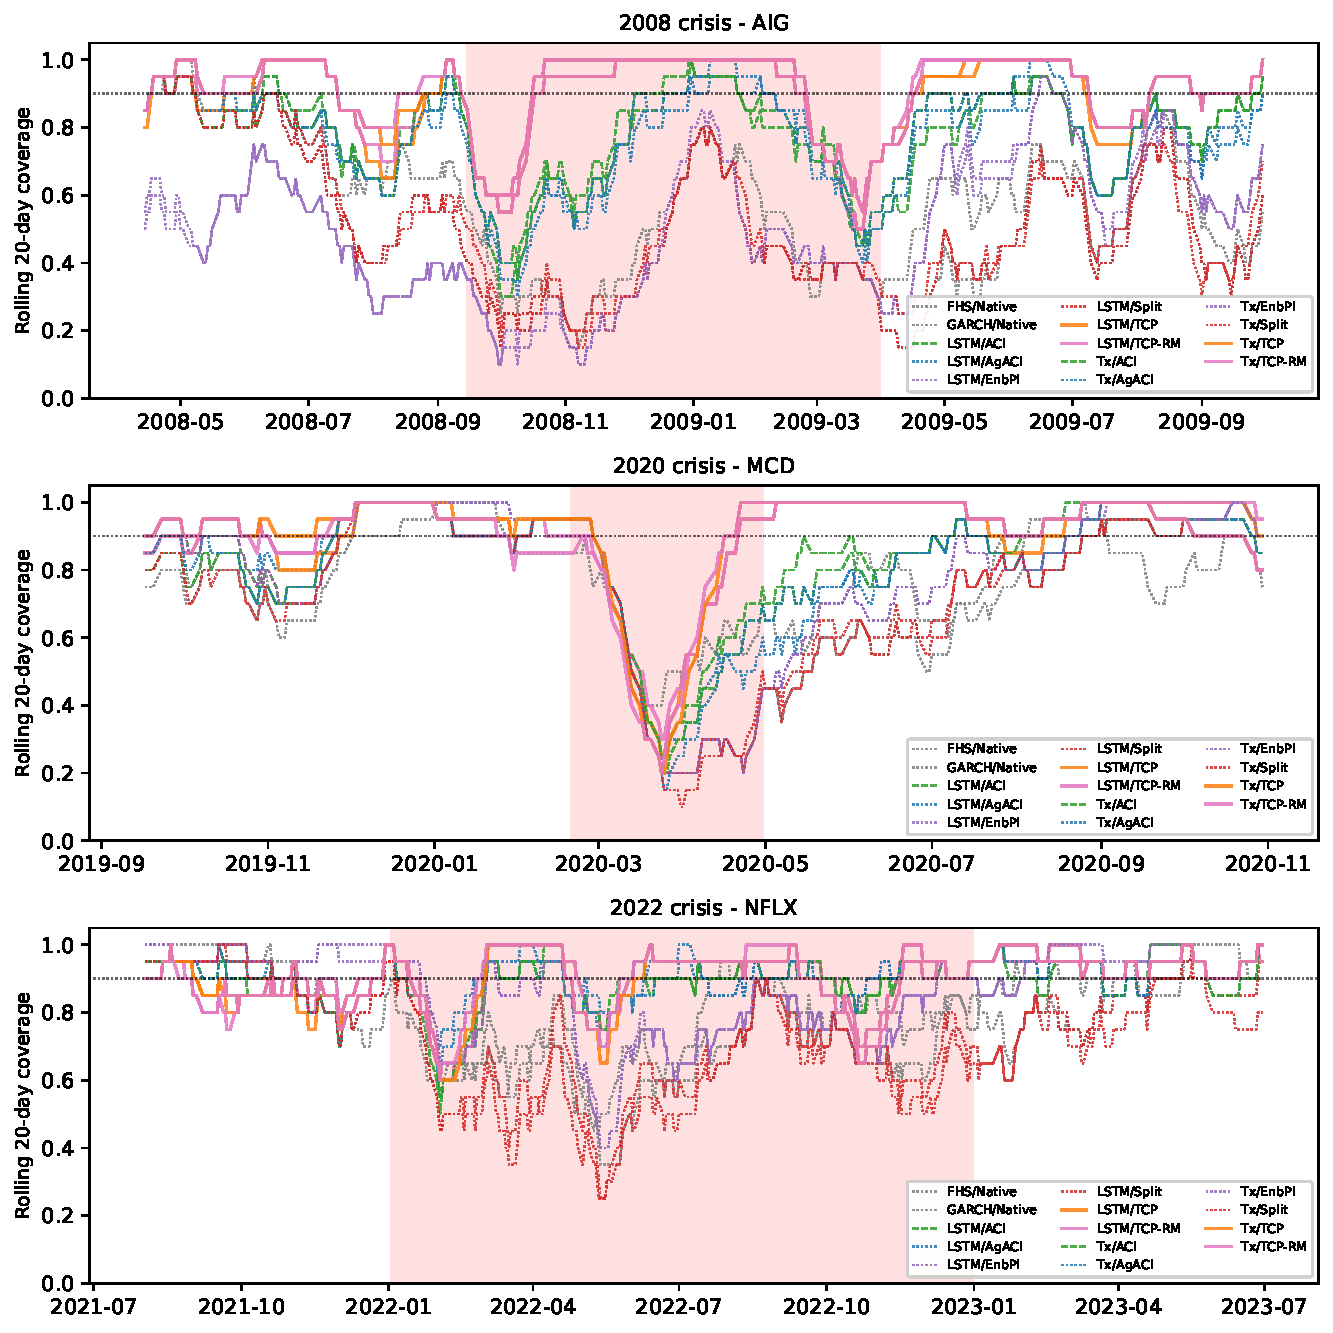
\includegraphics[width=\linewidth]{figures/rolling_coverage.pdf}
\caption{Rolling 20-day coverage averaged across tickers in each regime. Gray lines (GARCH-Roll, FHS) remain near the 0.90 nominal line (dotted) through the crisis windows (red shading). Conformal methods (green, orange) dip sharply at onset and recover slowly. Line style encodes wrapper type: solid = native, dashed = split, dotted = ACI, dash-dot = AgACI.}
\label{fig:rolling}
\end{figure}

\end{document}
